\section{Simulation}

A realistic model of the LTCC has been developed, describing the location and material composition of the support
box, the mirrors, PMTs, Winston cones, magnetic shields, the C$_4$F$_{10}$ gas, and the optical properties of the
gas and mirrors and WCs as a function of wavelength, see Ref.~\cite{sim-nim}.

As part of the re-scoping of the CLAS Cherenkov detector to detect pions (both positive and negative) instead of
negatively charged electrons, the optics of the mirrors needed to be tuned in order to optimize the LTCC response
for the angles of incidence for both positive and negative charges. This was accomplished by aligning the mirrors using
straight tracks (photons) originating from the target (placed at the center of the CLAS12 coordinate system), see
Section~\ref{sec:mirrorAlignment}.

The efficiency of light collection, critical for LTCC operations, is tied into precise mirror positioning.
The simulation has all the relevant details to make decisions in the LTCC optic design, including the
mathematical outline of the mirror shapes and the placement of the optics focal point: the target (common to all mirrors)
and the centers of the face of the PMTs.

%\begin{figure}
%	\centering
%	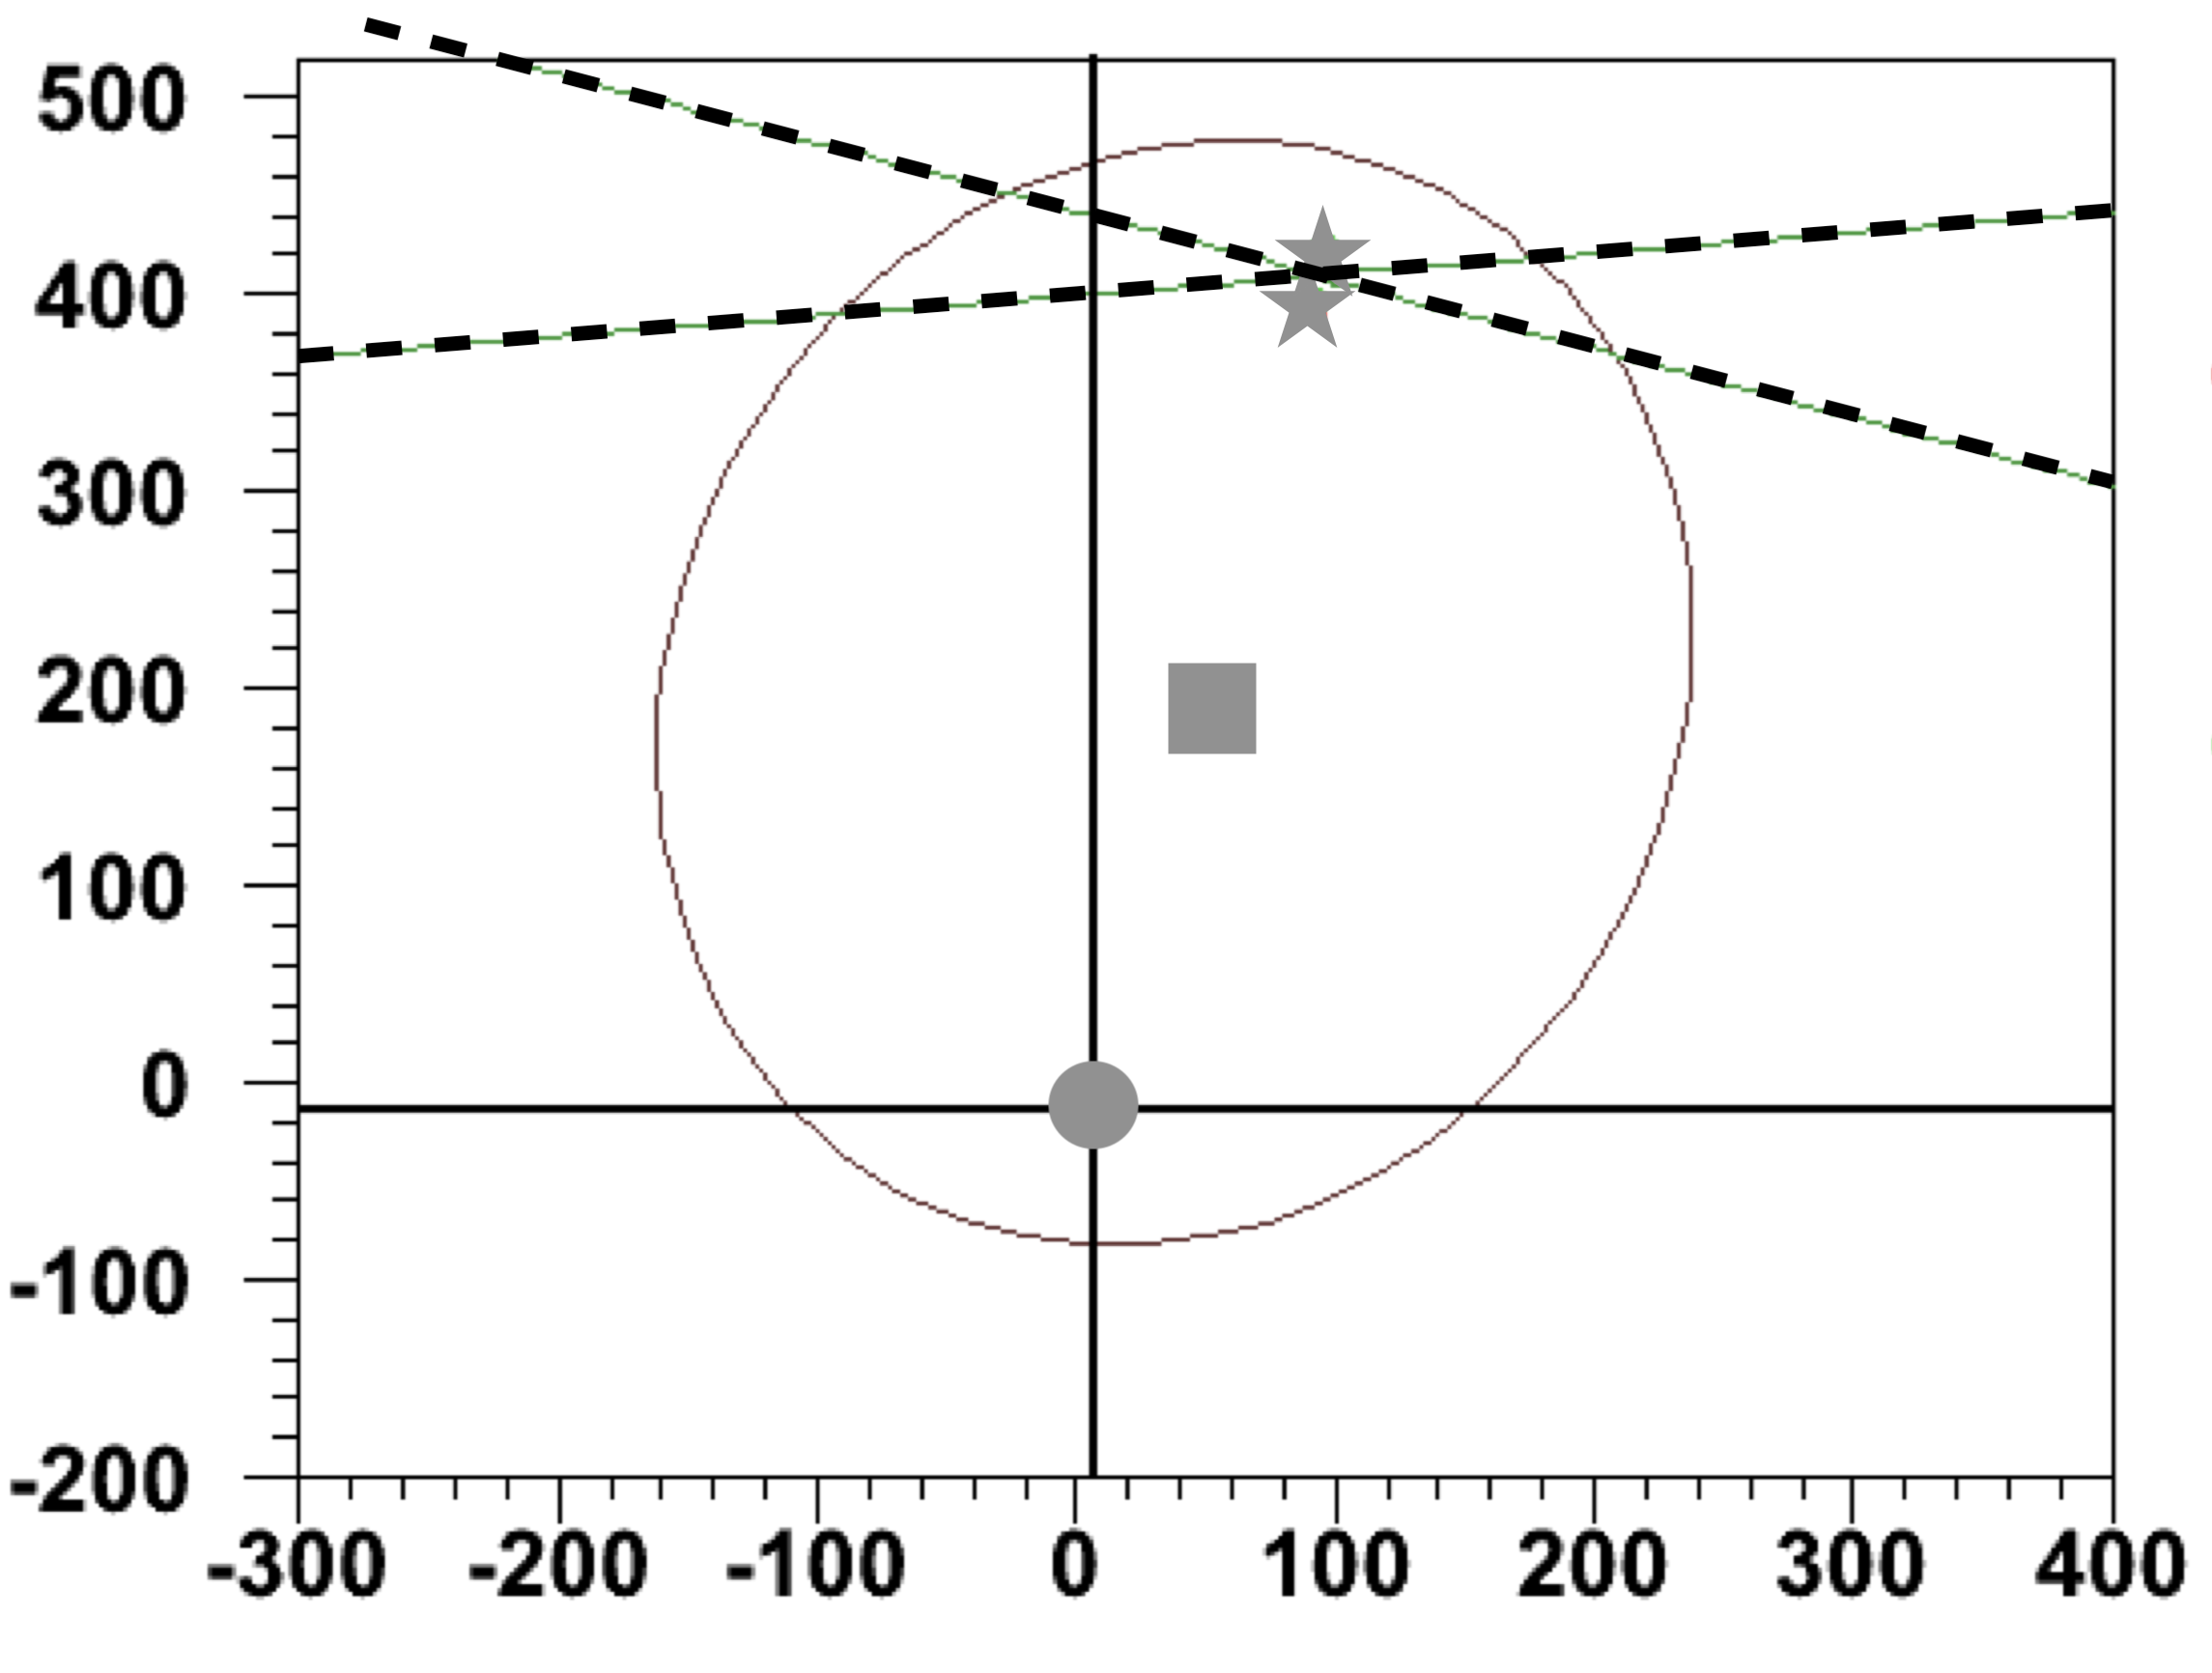
\includegraphics[width=0.98\columnwidth,keepaspectratio]{img/mirrorMath1.png}
%	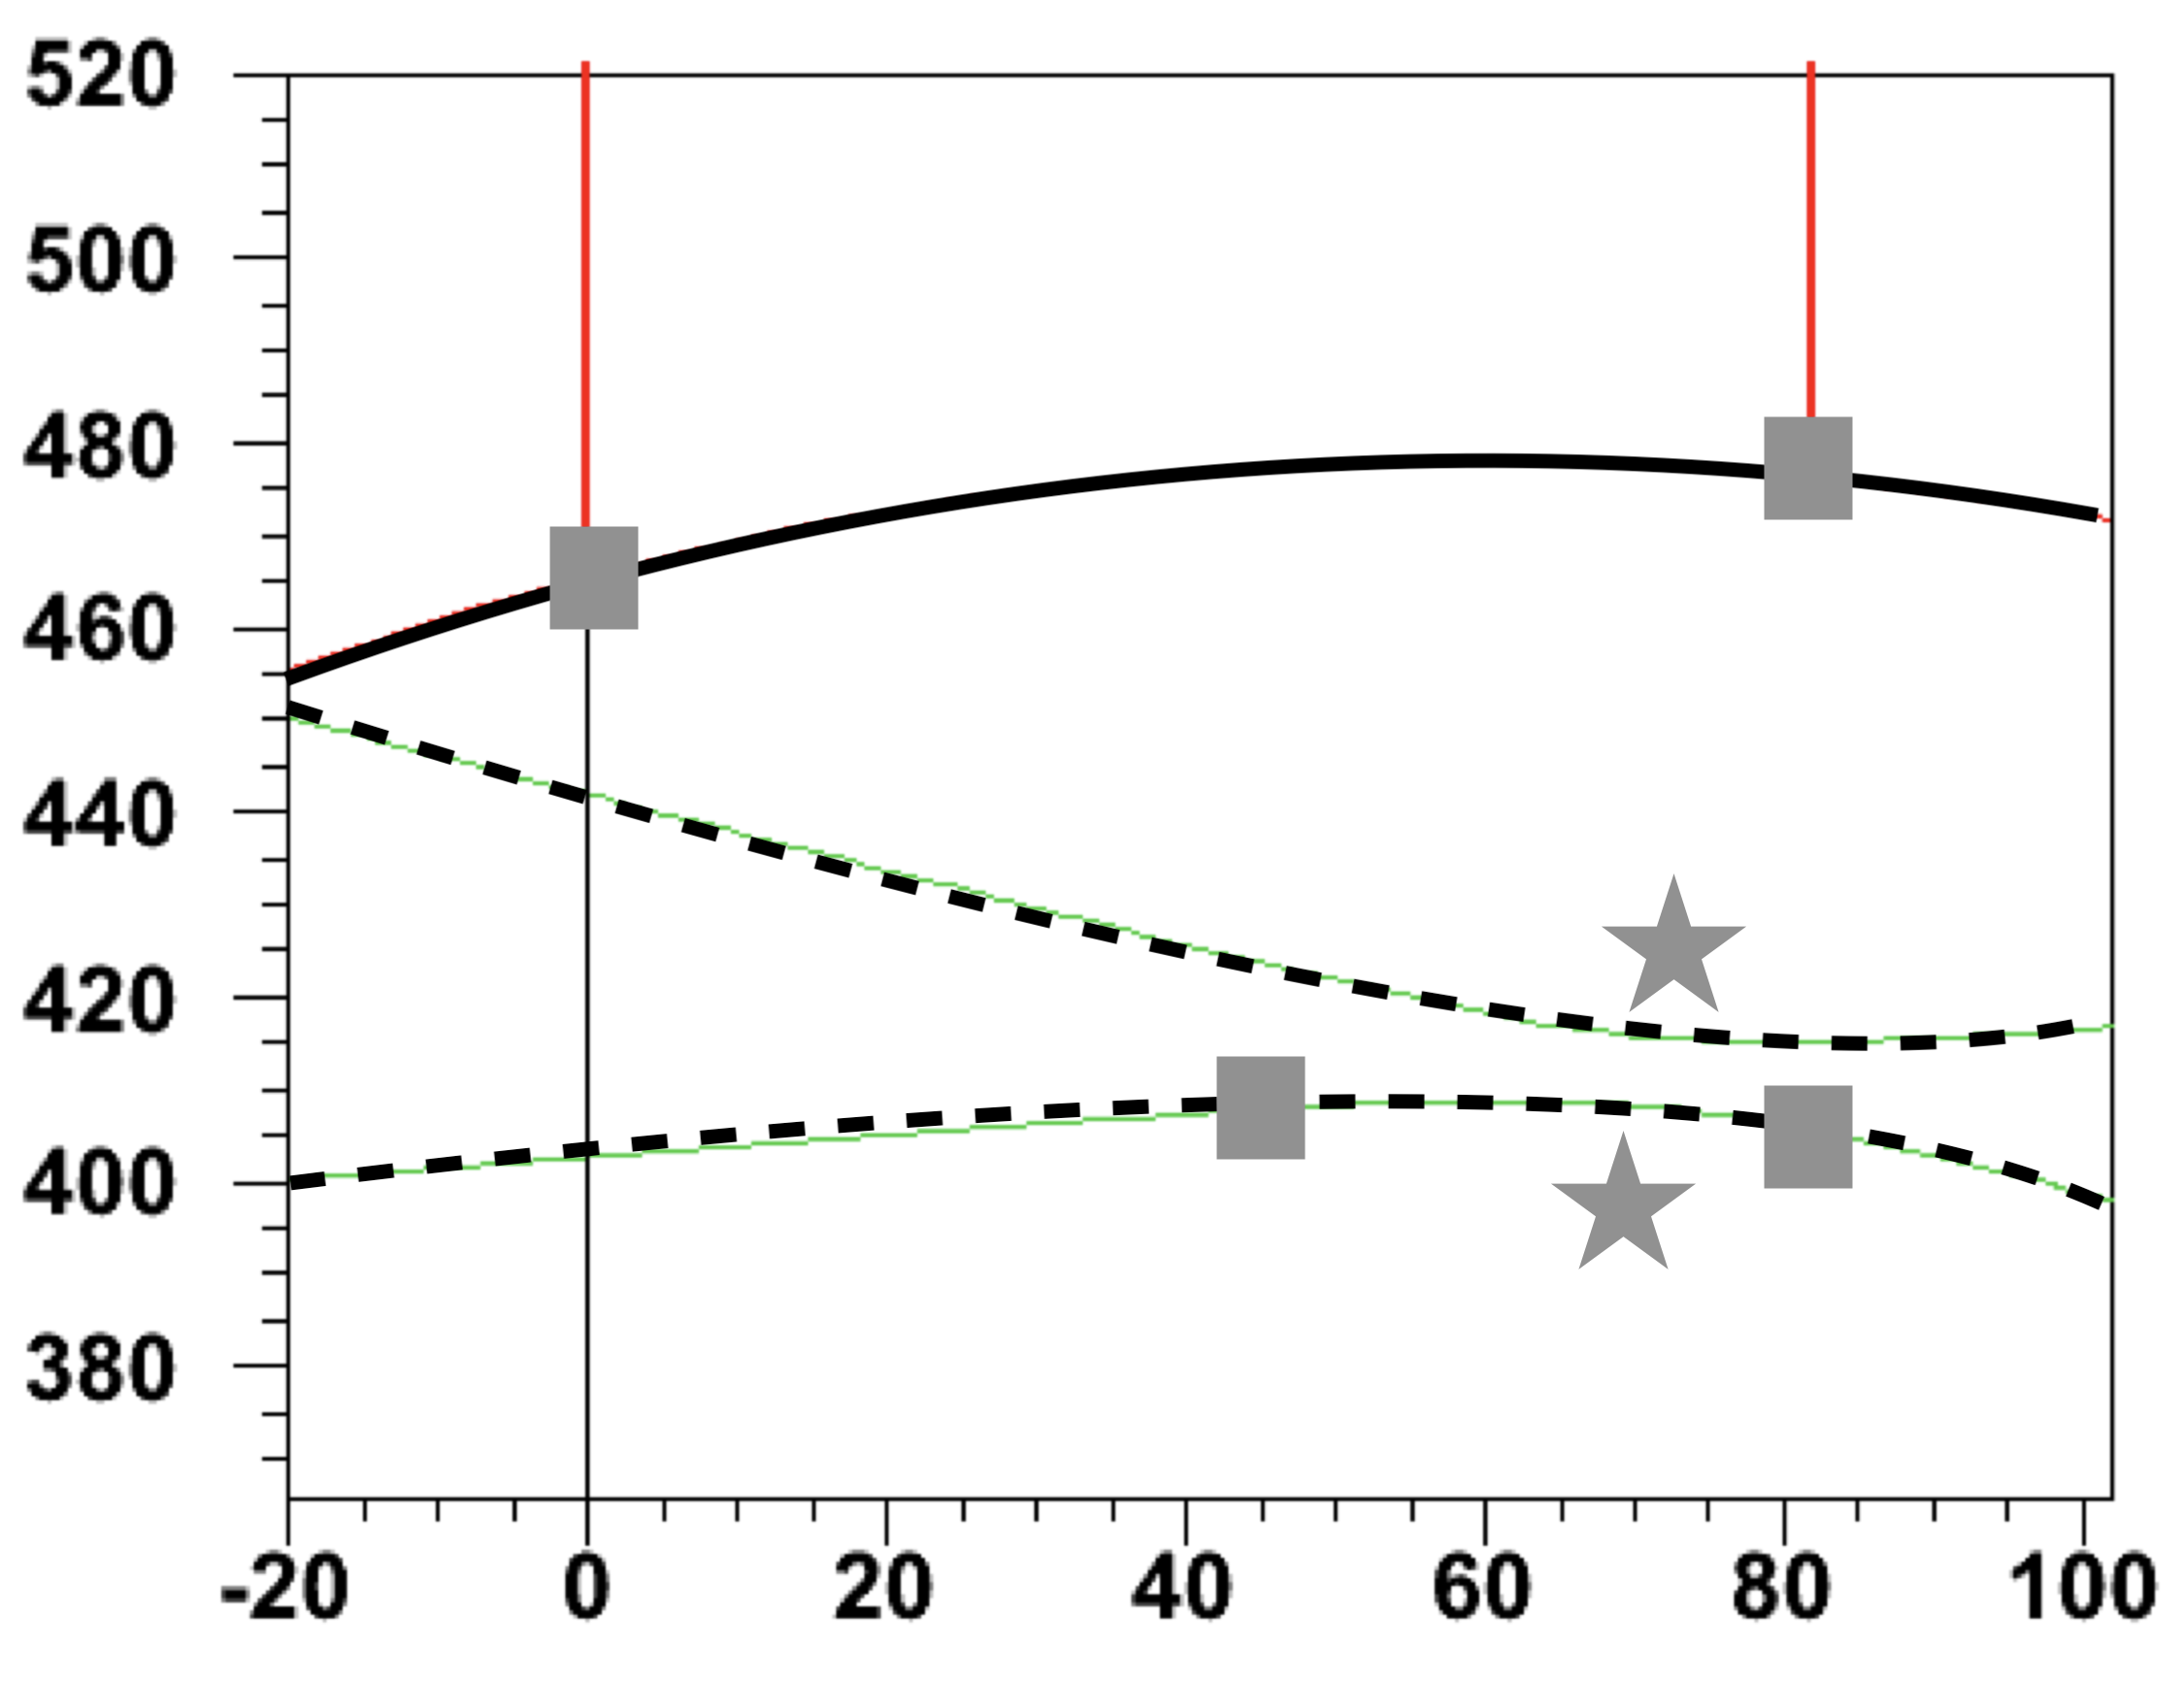
\includegraphics[width=0.98\columnwidth,keepaspectratio]{img/mirrorMath2.png}
%	\caption{The geometry of the LTCC mirrors is defined by functions describing an ellipse and a hyperbola. Top: the
%          ellipsoidal curve (solid line), with its center (square) and its focal points (circle at the origin, representing the
%          target, and the lower star). The two hyperbola curves, defined by the two focal points (stars, one coinciding
%          with the ellipse focal point and the other at the desired location of the PMT) are the dashed lines. The hyperbola
%          at the bottom is the one that defines the hyperbolic mirror. Bottom: zoomed in details of the top plot. The
%          squares represent the left and right mirror edges. These parameters are stored in databases and loaded in the
%          software modeling the LTCC mirrors in the GEMC simulation~\cite{sim-nim}.}
%	\label{fig:mirrorMath}
%\end{figure}

\subsection{Run Period Variations}

At the start of CLAS12 beam operations, there was not sufficient C$_4$F$_{10}$ gas to fill all sectors, so some LTCC
sectors were removed from the Forward Carriage. As they were installed or removed, any gas leaks were found and
fixed. These CLAS12 configuration changes are imported in GEMC as database variations of the simulation setup. The
default simulations only include sector 2 (S2), S3, S5, and S6, as the RICH detector~\cite{rich-nim} replaces the LTCC
boxes in S4 (and a second RICH detector will be installed in the S1 position in the near future). The variations are listed
in Table~\ref{tab:simVariations}.

\begin{table}
	\begin{center}
		\begin{tabular}{| l | c |}
			\hline \hline
			Run Period       & Sectors Installed and Gas \\
			\hline
			Default          & S2, S3, S5, S6, all C$_4$F$_{10}$    \\
			Spring 2018  & S2, S3, S6 (N$_2$), S5 (C$_4$F$_{10}$)  \\
			Fall 2018    & S3 (C$_4$F$_{10}$), S5 (N$_2$)          \\
			Spring 2018  & S3 (C$_4$F$_{10}$), S5 (C$_4$F$_{10}$) \\
			\hline \hline
		\end{tabular}
	\end{center}
	\caption{LTCC simulation variations for different CLAS12 run periods. Shown are the configurations of the
          LTCC boxes in the different sectors of the CLAS12 Forward Carriage for each run period and the gas that
          was used to fill the detectors.}
	\label{tab:simVariations}
\end{table}
